\documentclass{mcmthesis}
\mcmsetup{CTeX =false,   % 使用 CTeX 套装时,设置为 true
        tcn = 2121517, problem = A,
        sheet = true, titleinsheet =true, keywordsinsheet = true,
        titlepage =false, abstract = false}
\usepackage{palatino}
\usepackage{lipsum}
\usepackage{times}
\usepackage{geometry}
%===============设置正文和数学字体=============================
%有些字体需要安装一些字体文件,注意辨别。


\usepackage{graphicx}
\usepackage{subfigure}
%设置段落之间的距离,若不需要删除或者注释掉即可。
\setlength\parskip{.5\baselineskip}
\newtheorem{definition}{Definition}[section]
%\def\abstractname{Summary}%可修改摘要名称

\usepackage{indentfirst}
\setlength{\parindent}{2em}

\usepackage{chngpage}
\usepackage{array}
\usepackage{booktabs}
\usepackage{threeparttable}
\usepackage[numbers,sort&compress]{natbib}
%%% 实现参考文献标号在右上角
\newcommand{\upcite}[1]{\textsuperscript{\textsuperscript{\cite{#1}}}}
%然后引用的时候使用\upcite{}的格式(一般的正常引用格式为\cite{})

\usepackage{titletoc}
\titlecontents{section}[3cm]{\bf \large}{\contentslabel{2.8em}}{}{%
\titlerule*[0.5pc]{$\cdot$}\contentspage}%
\titlecontents{subsection}[4cm]{\normalsize}{\contentslabel{2.5em}}{}{%
\titlerule*[0.5pc]{$\cdot$}\contentspage}%
\titlecontents{subsubsection}[5.3cm]{\normalsize}{\contentslabel{3.0em}}{}{%
\titlerule*[0.5pc]{$\cdot$}\contentspage}%

\title{\large Traits and Environments: Factors Affecting Fungal Decomposition}
\author{ }


\date{\today}

\geometry{left=3.0cm,right=3.0cm}

\begin{document}
	
\begin{abstract}
	
The decomposition of ground litter and woody fibers is important in the global carbon cycle and fungi play a vital role in the process. In order to explore the specific role of fungi in the decomposition process, we start from several angles. One angle is  fungal traits, including hyphal extension rate(HER) and moisture tolerance(MT). Another is the influence of environmental factors, including temperature and moisture. Meanwhile, different fungal species will also affect each other’s growth and decomposition.

In response to the five requirements given , we have stated five questions to answer, and established two macroscopic models:Multi-fungal decomposition model and Decomposition model under environmental changes.

First of all, in the first model, to focus on the influence of the fungal traits and interactions on the decomposition rate(DR), we assume that environmental factors are constant. The two important direct influencing factors about DR are HER and MT. Based on data, we drew the curves of DR-HER and DR-MT, and determined their mutual relationships. With the help of the logestic model, we can determine HER. MT of one species in presence of several species can also be determined.With these two data, the population’s decomposition rate can be determined, fulfilling the first requirement.

Secondly, in order to consider the interactions among populations, we introduce suppression parameters to describe the competition model in the presence of multiple populations and the corresponding decomposition model, which solves the second problem. Meanwhile,with further analysis, we described the short- and long-term trends of the entire population and answered the first half of the third problem.

Then, in order to solve the next problem, we introduced environmental factors and established the second model. Environmental factors are mainly reflected in temperature(T) and moisture(M), so we draw HER-T and HER-M curve and analyzes the relationship between moisture and moisture tolerance. Then we analyzed the sensitivity of the population to environmental fluctuations , answering the third question.

Next, in order to solve the fourth problem, we introduced a new function to determine the competitive ranking of the population in different environments, thereby determining their advantages and disadvantages. In particular, we selected six populations and five typical environments to explore this.

Finally, we combined the two models to compare the decomposition efficiency and environmental adaptability of a single population and multiple populations.Thus the impact of population diversity is predicted, answering the fifth question.So far, we have completed the establishment of two models and met the five requirements. At the end of the article, we analyzed the sensitivity and stability of the model with the strengths and weaknesses.
\begin{keywords}
	Fungi, Decomposition Rate, Hyphal Extension Rate, Moisture Tolerance, Environmental Changes, Biodiversity, Logistic
\end{keywords}
\end{abstract}
\maketitle
%\pagestyle{empty}
\newpage                                                          %
%==================================================================
%====================生=成=目=录===================================
\begin{adjustwidth}{-1cm}{0cm}

\setcounter{tocdepth}{3}
\thispagestyle{empty}
\tableofcontents                                                  %

\end{adjustwidth}


\newpage

\pagestyle{fancy}

\setcounter{page}{1}
\section{Introduction}
\subsection{Background}

The carbon cycle is a significant component for life on the earth,which describes the process of the exchange of carbon throughout the geochemical cycle of the Earth.Part of the carbon cycle includes the decomposition of compounds, allowing carbon to be renewed and used in other forms. One key component of this part of the process is the decomposition of plant material and woody fibers.

The key agents in decomposition are fungi.Recent research has indicated that the rates of decomposition are determined by fungi traits.The growth rate of the fungus and the fungus’ tolerance to moisture are two major traits of a fungus we tend to focus on.

\subsection{Problem Restatement}
\begin{itemize}
	\item
	How to build a model to determine the decomposition process of fungi?
	\item
	How to describe the interactions between different species of fungi in the model?
	\item
	Provide an analysis of the model and describe the dynamics of the interactions in short and long-term trends. Does the analysis examine the sensitivity to rapid fluctuations and determine the overall impact over variation of weather patterns?
	\item
	How to predict the relative advantages and disadvantages for each fungal species and its combinations likely to persist over different environments?
	\item
	How to describe the impact of fungal population diversity on ground litter decomposition?And how to predict the role of population diversity in a changing environment?
\end{itemize}

\section{Assumptions and Justification}

\begin{itemize}
\item 
The direct influencing traits of the decomposition rate are Hyphal extension rate and Moisture tolerance, and other influencing traits all indirectly affect the decomposition rate by influencing the changes of the above two traits.

$\hookrightarrow$Justification:In the introduction, the question requires us to focus on the impact of these two features on the decomposition rate and provide the relevant change curve. Based on the fact that all the characteristics of the colony are related to each other, we assume that all the characteristics of the colony involved in the whole model affect the decomposition rate by affecting the two characteristics of Hyphal extension rate and Moisture tolerance.

\item 
The model does not consider the rate change caused by the chemical mechanism change of the decomposition process itself,such as enzyme activity,etc.

$\hookrightarrow$Justification:The changes in the chemical mechanism of the decomposition process involve complex chemical reaction equations and the consideration of the activation energy of the reaction. It belongs to the category of chemical biology and has little impact on modeling issues. We have ignored them for modeling considerations.

\item 
All strains in the model have an initial quantity, which is 10\% of the maximum quantity that the strain can grow alone under the resource-limited environmental conditions.

$\hookrightarrow$Justification:To analyze the decomposition rate, there must be enough colonies as a support. The entire model is related to the number of colonies, so we have to make assumptions about the initial value of the number. At the same time, this is also in line with the actual situation where the spoilage is decomposed by initial fungi.

\item 
The model focuses on the mid-term of the whole litter corruption process, and uses the mid-term situation to represent the entire decomposition process.

$\hookrightarrow$Justification:As stated in the requirements, although the various processes of corruption are different, the environmental time period analyzed by our model is generally in the middle stage of corruption where it grows vigorously and decomposes rapidly, so we assume as above.

\item
Both the growth and climate change of the colony are predictable.

$\hookrightarrow$Justification:Although there will be small-probability emergencies in growth climate change, we believe that it is predictable in the longer time and larger range of the model, and the conclusions obtained are suitable for a universal range.

\item
All data cited in the article are accurate.

$\hookrightarrow$Justification:All data come from professional databases and academic papers, and are obtained from experimental data, which can be considered true and accurate.

\end{itemize}

\section{List of Notation}

\begin{table}[h]
	\centering
	\caption{The List of Notation}
	\begin{tabular}{p{.1\textwidth}p{.8\textwidth}m{.4\textwidth}}
		\hline
		Symbol& Meaning \\
		\hline
		$T$      & Temperature\\
		$M$      & Moisture\\
		$HER$	 & Hyphal extension rate\\
		$DR$     & Decomposition rate\\
		$MT$     & Moisture tolerance\\
		$t$      & Time\\
		$r$      & Growing rate\\
		$N_{0}$  & Maximum capacity\\
		$N(t)$   & Population density\\
		$ES$     & Environmental sensitivity\\
		\hline
	\end{tabular}
\end{table}

\section{Multi-fungal decomposition model}
Firstly,we consider a model of the decomposition of litter by a variety of fungi when the temperature and humidity are kept roughly constant. Regarding decomposition, the most important thing is to determine the decomposition rate. In a constant environment, we use the logistic population growth model to determine the growth rate of the population, determine the moisture tolerance by the population’s competitive ranking and moisture niche width in this environment, and then determine the decomposition rate by these two variables to establish the entire Multi-fungal decomposition model.

\subsection{Analysis of growth rate based on logistic model}
According to the law of population growth, in a constant environment, due to growth data and environmental constraints, the population cannot grow indefinitely, and its hyphal extension rate will increase first and then decrease. If the density growth rate of the relative population density under the condition of unlimited resources is $r$, $r$ is affected by the environment, and the maximum density that the population can reach under resource constraints is $N_{0}$, the rate of the density growth rate affected by the population density $N$ is$\frac{r}{N_{0}}N$,its differential equation is as follow:
\begin{equation} 
	\left\{ 
	\begin{aligned}
		\frac{dN(t)}{dt}&=\frac{r}{N_{0}}N(N_{0}-N)
		\\N(0)&=0.1N_{0}
	\end{aligned}
	\right. 
\end{equation} 

Based on formula (1), the following left logistic growth curve of population density can be drawn, and the corresponding changes in the hyphal extension rate can be obtained.
\begin{figure}[h]
	\centering{
		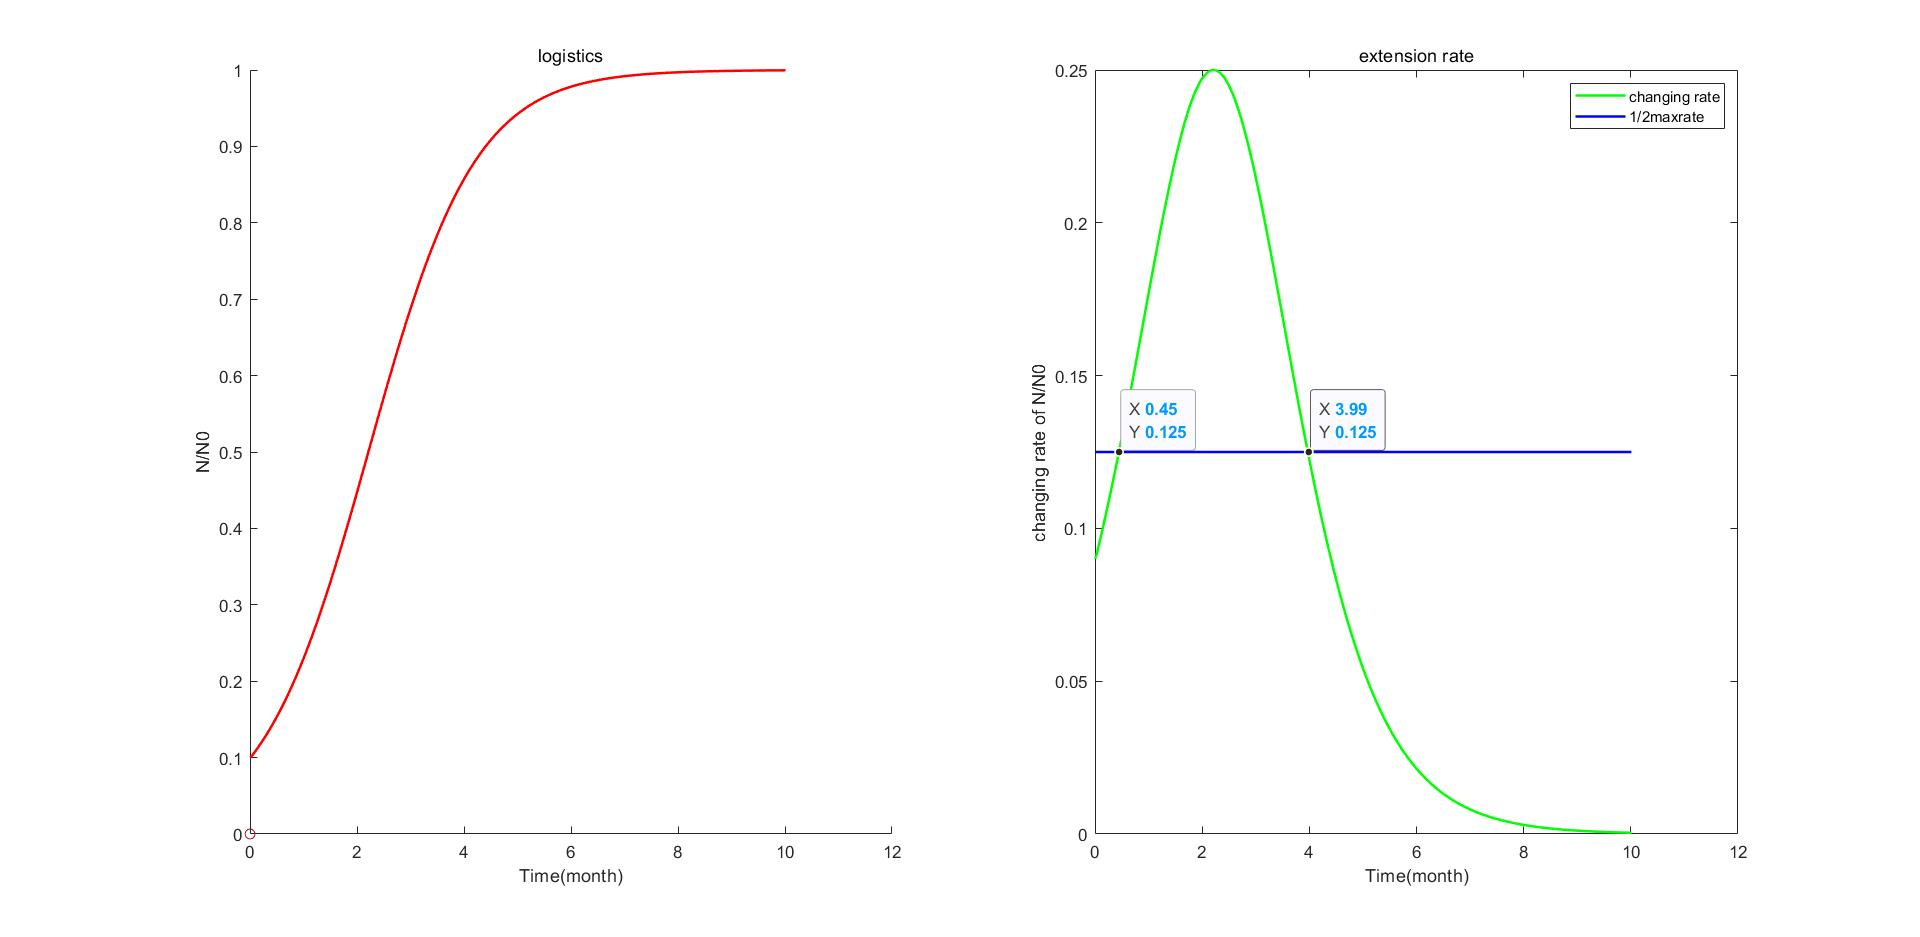
\includegraphics[width=0.8\textwidth]{./picture/logistic.jpg}}
	\caption{logistic growth}
\end{figure}

Since the moisture niche width is set within the range of 50\% of the maximum rate $\frac{1}{4}N_{0}r$ of the hyphal extension rate, it is assumed that the period greater than 50\% is the rapid growth stage in the middle of decomposition, and the average value of the hyphal extension rate in this stage It can be considered as the hypohal extension rate in the later model. According to the curve on the upper right of the hypohal extension rate, the average rate can be calculated as $0.2022N_{0}r$ by the integral method.


\subsection{Decomposition rate model with respect to HER and MT}
%It can be seen from the discussion above that the woody decomposition rate is affected by hyphal extension rate and Moisture tolerance.
In a specific environment where multiple fungal populations exist, the growth rate of a population can be obtained by the above-mentioned logistic model, and its moisture tolerance is also determined and unchanged (the specific determination method is described in the next section). Therefore, it can be considered that the hyphal extension rate and moisture niche width of a certain group in this environment are known, then the decomposition rate can be obtained by considering the relationship model between the decomposition rate, the growth rate and the moisture tolerance, and it is determined that it is effective for ground litter and woody fibers' decomposition situation.

To get the relationship, we have to build a function, considering the general laws in the case of multiple data. The independent variables are hyphal extension rate ($HER$) and moisture tolerance ($MT$), the dependent variable is the decomposition rate ($DR$), and the function relation is set as follow:
\begin{equation} 
	DR=f(HER,MT)
\end{equation}

To get the relationship, we need to use relevant data (see the attachment for the data). Since the data is obtained under the control variables, we are also analyzing under the assumption that one of the variables is fixed.

Firstly, assume that the moisture tolerance is stable. In the case of a single specie, the value can be regarded as $d_{0}$. The $HER$ and the corresponding $DR$ at different temperatures in the data are introduced, and the basic logarithmic relationship between the two can be determined by fitting on the scatter plot. Further processing can get the relationship diagram as shown below.
\begin{figure}[h]
	\centering{
		\includegraphics[width=0.8\textwidth]{./picture/DR-HER.jpg}}
	\caption{DR-HER}
\end{figure}

From the above figure, the relationship between $DR$ and $HER$ at different temperatures can be described as follow:
\begin{equation} 
	DR=f(HER,0)=k_{1}ln(HER)+c_{1}
\end{equation}
where the values of $k_{1}$ and $c_{1}$ are related to temperature. Since the environment we set is constant, the values of these two coefficients are constant at the corresponding temperature.

Then assume that the value of HER is stable, set to a constant $h_{0}$. Introduce the MT of various groups in the data and the corresponding decomposition rate, and by fitting on the scatter plot, it can be determined that the two are basically exponential. Further processing can get the relationship diagram as shown below.
\begin{figure}[h]
	\centering{
		\includegraphics[width=0.8\textwidth]{./picture/DR-MT.jpg}}
	\caption{DR-MT}
\end{figure}

From the above figure, the relationship between DR and MT under constant HER can be described as follow: 
\begin{equation} 
	DR=f(h_{0},MT)=c_{2}e^{k_{2}MT}
\end{equation}

Based on the discussion above, we assume that:
\begin{equation} 
	c_{2}=g_{1}(HER), k_{1}=h_{1}(MT)
\end{equation}
and 
\begin{equation} 
	k_{2}=g_{2}(HER), c_{1}=h_{2}(MT)
\end{equation}

Consider within a certain range,we have:
\begin{equation} 
	Cov(HER,MT)=0
\end{equation}
then we get
\begin{equation} 
	\frac{{\partial}DR}{{\partial}HER}=c_{2}e^{k_{2}MT}g_{2}'+e^{k_{2}MT}g_{1}'=\frac{k_{1}}{HER}
\end{equation}
and
\begin{equation} 
	\frac{{\partial}DR}{{\partial}MT}=log(HER)h_{1}'+h_{2}'=c_{2}k_{2}e^{k_{2}MT}
\end{equation}

We solve that $DR$ linearly tends to
\begin{equation} 
	(m_{1}log(HER)+m_{2})n_{1}e^{n_{2}MT}
\end{equation}
\subsection{Analysis of multiple fungus}
In order to analyze this model more accurately, we introduce the following variables.
\begin{table}[h]
	\centering
	\caption{notation in this part}
	\begin{tabular}{p{.1\textwidth}p{.8\textwidth}m{.4\textwidth}}
		\hline
		Symbol& Meaning \\
		\hline
		$CR$     & Competitive ranking\\
		$W$      & Absolute value of moisture niche width\\
		$w$      & Relative value of moisture niche width\\
		$a_{i}(t)$  & Relative content of the i-th fungus\\
		$s_{ij}$ & Inhibition rate of the i-th fungus on the j-th fungus\\
		$C_{K}$  & solution vector,where $C$ is a n-tuple vector\\
		\hline
	\end{tabular}
\end{table}

\subsubsection{Data of moisture tolerance}
In the presence of multiple fungi, the competitive ranking and moisture niche width of each fungus population can be obtained by analyzing the characteristics of fungi. The competitive ranking is the value in $[0,1]$, and the moisture niche width is the real value. In order to get the moisture tolerance of the two uniformly, we need to process the data.

The processing method is to convert the moisture niche width into a value in $[0,1]$ according to the relative level. To this end, we take out the maximum $W_{max}$ and minimum $W_{min}$ of the true value of the moisture niche width in all populations, and assume a linear relationship, so that the relative moisture niche width w is obtained from the $W$ value of each population: 
\begin{equation} 
	w=\frac{W-W_{min}}{W_{max}-W_{min}}
\end{equation}

According to the definition of moisture tolerance, we have theexpression: 
\begin{equation} 
	MT=CR-w
\end{equation}

Substituting the $CR$ and $w$ corresponding to different populations, the $MT$ value of the population can be obtained, and its range is $[-1,1]$.
\subsubsection{Multi-fungal Competitive model}
In the presence of n species of fungi, their growth will be affected by mutual competition based on their different moisture resistance. By introducing differential equations, we can establish their own growth models under multi-fungal competition. For the i-th fungus, $a_{i}(t)$ represents the ratio of the maximum content at time $t$ relative to the maximum content that can be grown alone in the environment,
\begin{equation} 
	a_{i}(t)=\frac{N_{i}}{N_{0i}}
\end{equation}
$r_{i}$ represents the growth rate under the environment, and $s_{ij}$ as a parameter of competition and mutual influence is reflected by moisture resistance,
\begin{equation} 
	s_{ij}=1-\frac{MT_{j}-MT_{i}}{MT_{max}-MT_{min}}
\end{equation}
So we can get the differential equation about the growth of the i-th fungus
\begin{equation} 
	\left\{ 
	\begin{aligned}
		\frac{da_{i}(t)}{dt}&=r_{i}(1-\sum_{j=1}^{n}s_{ji}a_{j}(t))a_{i}(t)
		\\a_{i}(0)&=0.1
	\end{aligned}
	\right. 
\end{equation} 

Assume that solution vector is $C_{K}=\{C_{1},C_{2},C_{3},\cdots\}$,we estimate that predictable regular time is $t_{total}$,which is roughly 122days,and
\begin{equation} 
	dt=\frac{t_{total}}{K}
\end{equation} 
where the larger the K, the more accurate the result,we assume that the program simulation time is 1000.

We get the numerical recursion from the differential equation:

\begin{equation}
	C_{x+1}=C_{x}+\{(r-C_{x}^{T}S){\cdot}C_{x}^{T}{\cdot}r^{T}dt\}^{T}
\end{equation}
and the expression for each term:
\begin{equation}
	C_{x}(m)=a_{m}(x-1)dt
\end{equation} 
where $x=2,3,4,\cdots$

\begin{figure}[h]
	\centering{
		\includegraphics[width=0.8\textwidth]{./picture/competition.jpg}}
	\caption{competition}
\end{figure}

The above is the image of the competition relationship between the populations obtained based on the previously discussed algorithm and the simulated data. It can be clearly seen from the figure that there are competition and other relationships between different populations, and the number of populations will change with time.

We will analyze the stability and sensitivity of this model later.
\subsection{Interaction and Dynamic changes}
Since the overall resources for fungal growth in an environment are limited, we start from biological knowledge and believe that multiple fungal populations are in a competitive relationship with each other in the environment. Competitive ranking of a population in the entire multi-group is manifested as competitive ranking, which has a positive correlation with moisture tolerance. Therefore, in the above model, we obtain the inhibition parameter sij of the competition among the populations through moisture resistance, so as to describe the competition relationship.

Our model curve diagram is to take out six species of bacteria with different moisture tolerance, and regard their initial quantity as the same (all are 0.1 of the maximum content), and the six population numbers obtained from the analysis of competition relationship vary with each other. Time change relationship. According to the change relationship, we can analyze the change trend of the multi-fungi population. 

In the short term, since the populations are the same at the beginning, there is no obvious competition between them at the beginning. The populations of all populations will increase, and the fungal populations with higher competition levels (that is, stronger moisture tolerance) will grow faster. The growth is fast, the decomposition rate is relatively fast, and the low population is correspondingly slow. 

From a long-term perspective, due to the fast growth rate of populations with high competition levels, its inhibitory effect on populations with low competition levels will be obvious, and the number of low-level populations will therefore have a downward trend, eventually tending to zero. Therefore, the long-term trend of the development of the entire multi-fungal population is that the high-competitive populations are left, and the low-ranking populations may die.


\section{Decomposition model under environmental changes}
Now we consider adding environmental factors to the above model to analyze the multi-fungal decomposition model under environmental changes. Among the many environmental factors, we emphatically consider the influence of temperature and humidity on the decomposition model. With temperature and humidity as the main parameters, combined with the climate change of multiple specific environments, we will make a simple prediction of the population development in a specific environment, and use this to briefly explain the significance of fungal population diversity.
\subsection{Functions between several important variables}
Based on the basic assumptions and the above model, we believe that the decomposition rate is directly affected by the hypohal extension rate and the moisture tolerance, and can be determined by both. Therefore, regarding the influence of temperature and humidity on the decomposition rate, we first consider the influence of temperature and humidity on the hypohal extension rate and moisture tolerance
\subsubsection{HER-T and HER-M functions}
By consulting the literature, under the establishment of the relevant model, we obtained the relationship between temperature and hyphal extension rate under other conditions unchanged as follow,
\begin{equation}
	HER=HER_{max}{\times}(\frac{T_{max}-T}{T_{max}-T_{opt}})^{\alpha}{\times}e^{-{\alpha}(\frac{T_{max}-T}{T_{max}-T_{opt}}-1)}
\end{equation} 
Where $HER(T)$ is the hyphal extension rate at temperature $T$, $HER_{max}$ is the hyphal extension rate at optimal temperature Topt, Tmax is the maximum temperature at which the colony can grow normally, and $\alpha$ is a constant. 

We can draw the $HER-T$ relationship curve by knowing the corresponding data of certain populations.
\begin{table}[h]
	\centering
	\caption{HER-T}
	\begin{tabular}{p{.4\textwidth}p{.15\textwidth}p{.12\textwidth}p{.12\textwidth}p{.05\textwidth}}
		\hline
		Fungal species&$HER_{max}$&$T_{opt}$&$T_{max}$&$\alpha$ \\
		\hline
		Tetracladium marchalianum & 96.4 & 20 & 28.0 & 3.1\\
		Alatospora acuminata & 106.7 & 23 & 32.2 &2.5\\
		Heliscus lugdunensis & 100.2 & 22.5 & 42.4 &7.1\\
		\hline
	\end{tabular}
\end{table}
\begin{figure}[h]
	\centering{
		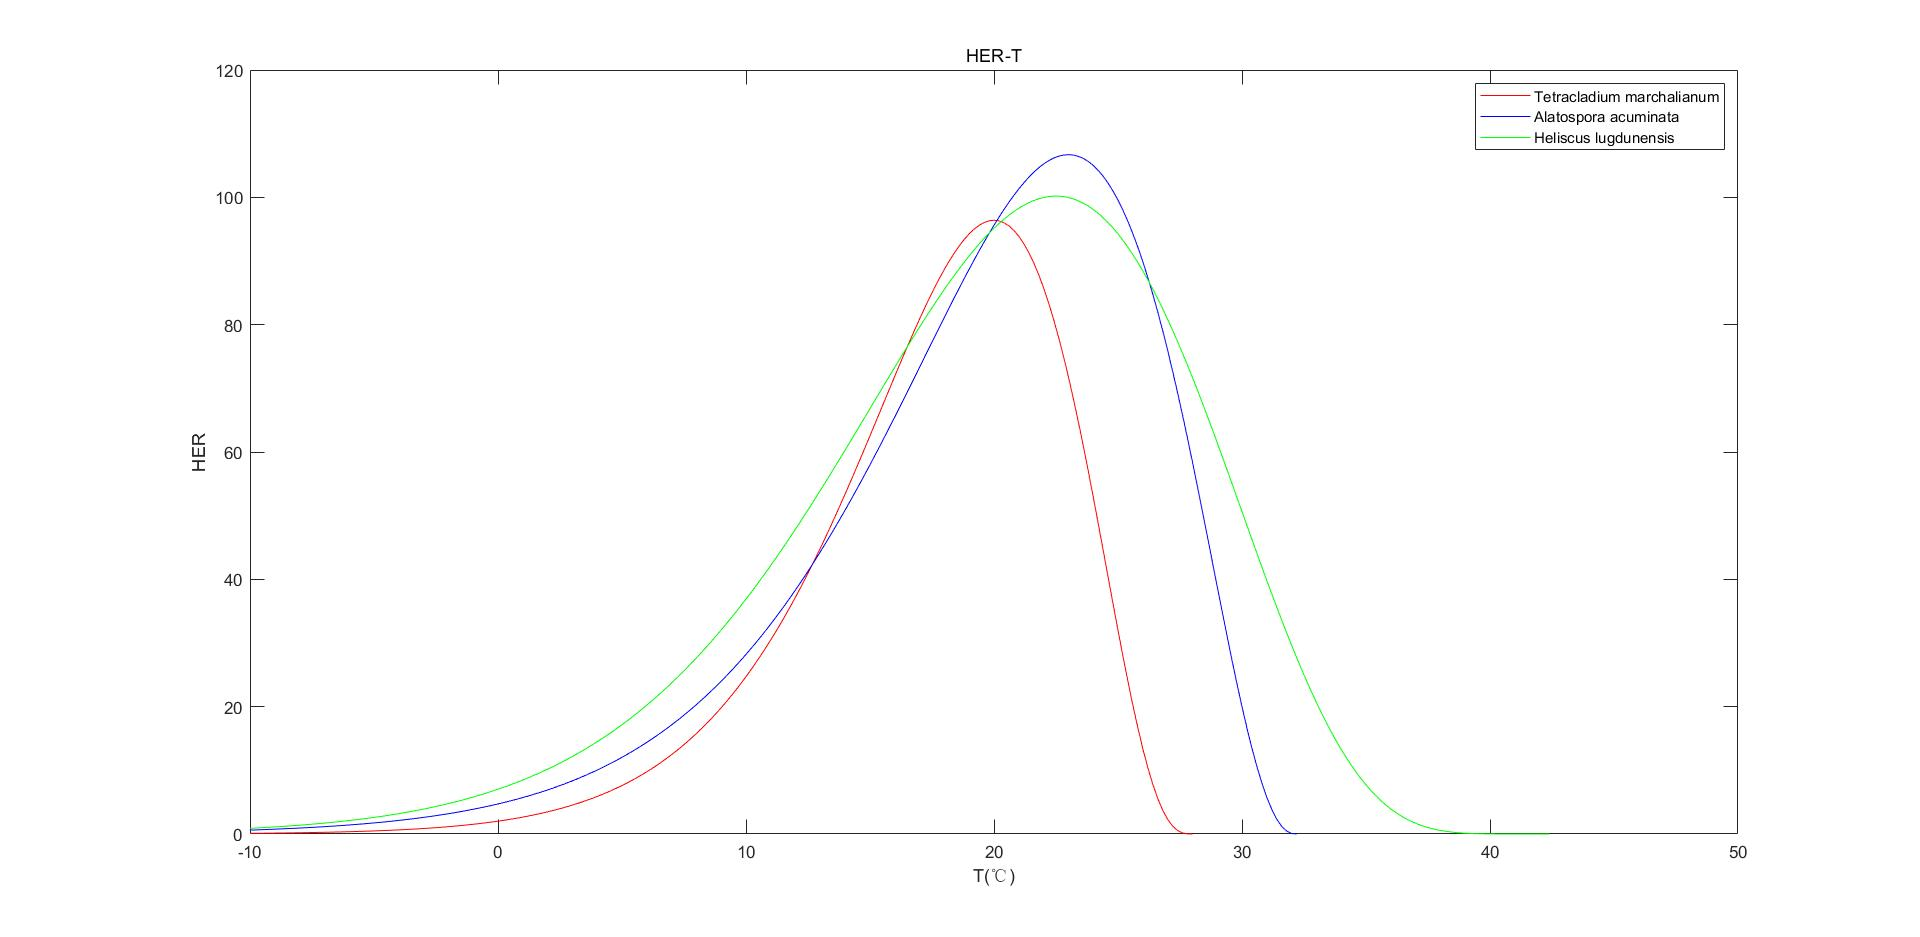
\includegraphics[width=0.8\textwidth]{./picture/HER-T.jpg}}
	\caption{HER-T}
\end{figure}

Similarly, for the relationship between humidity and hyphal extension rate, according to related literature, the curve relationship is similar to temperature. Under other conditions unchanged, the relationship is as follow,
\begin{equation}
	HER=HER_{max}{\times}(\frac{M_{max}-M}{M_{max}-M_{opt}})^{\beta}{\times}e^{-{\beta}(\frac{M_{max}-M}{M_{max}-M_{opt}}-1)}
\end{equation} 
Where $HER(M)$ is the hypohal extension rate under humidity $M$, $HER_{max}$ is the hypohal extension rate under optimal moisture $M_{opt}$, $M_{max}$ is the maximum temperature at which the colony can grow normally, generally $0$, and $\beta$ is a constant. 

Knowing the corresponding data of certain populations, we can draw the $HER-M$ relationship curve.
\begin{table}[h]
	\centering
	\caption{HER-M}
	\begin{tabular}{p{.4\textwidth}p{.15\textwidth}p{.12\textwidth}p{.12\textwidth}p{.05\textwidth}}
		\hline
		Fungal species&$HER_{max}$&$M_{opt}$&$M_{max}$&$\beta$ \\
		\hline
		Armillaria\_gallica\_FP102531\_C6D & 39.0 & -0.89 & 0.0 & 2.7\\
		Alatospora acuminata & 56.8 & -0.78 & 0.0 &3.5\\
		Heliscus lugdunensis & 36.1 & -0.92 & 0.0 &5.2\\
		\hline
	\end{tabular}
\end{table}

\begin{figure}[h]
	\centering{
		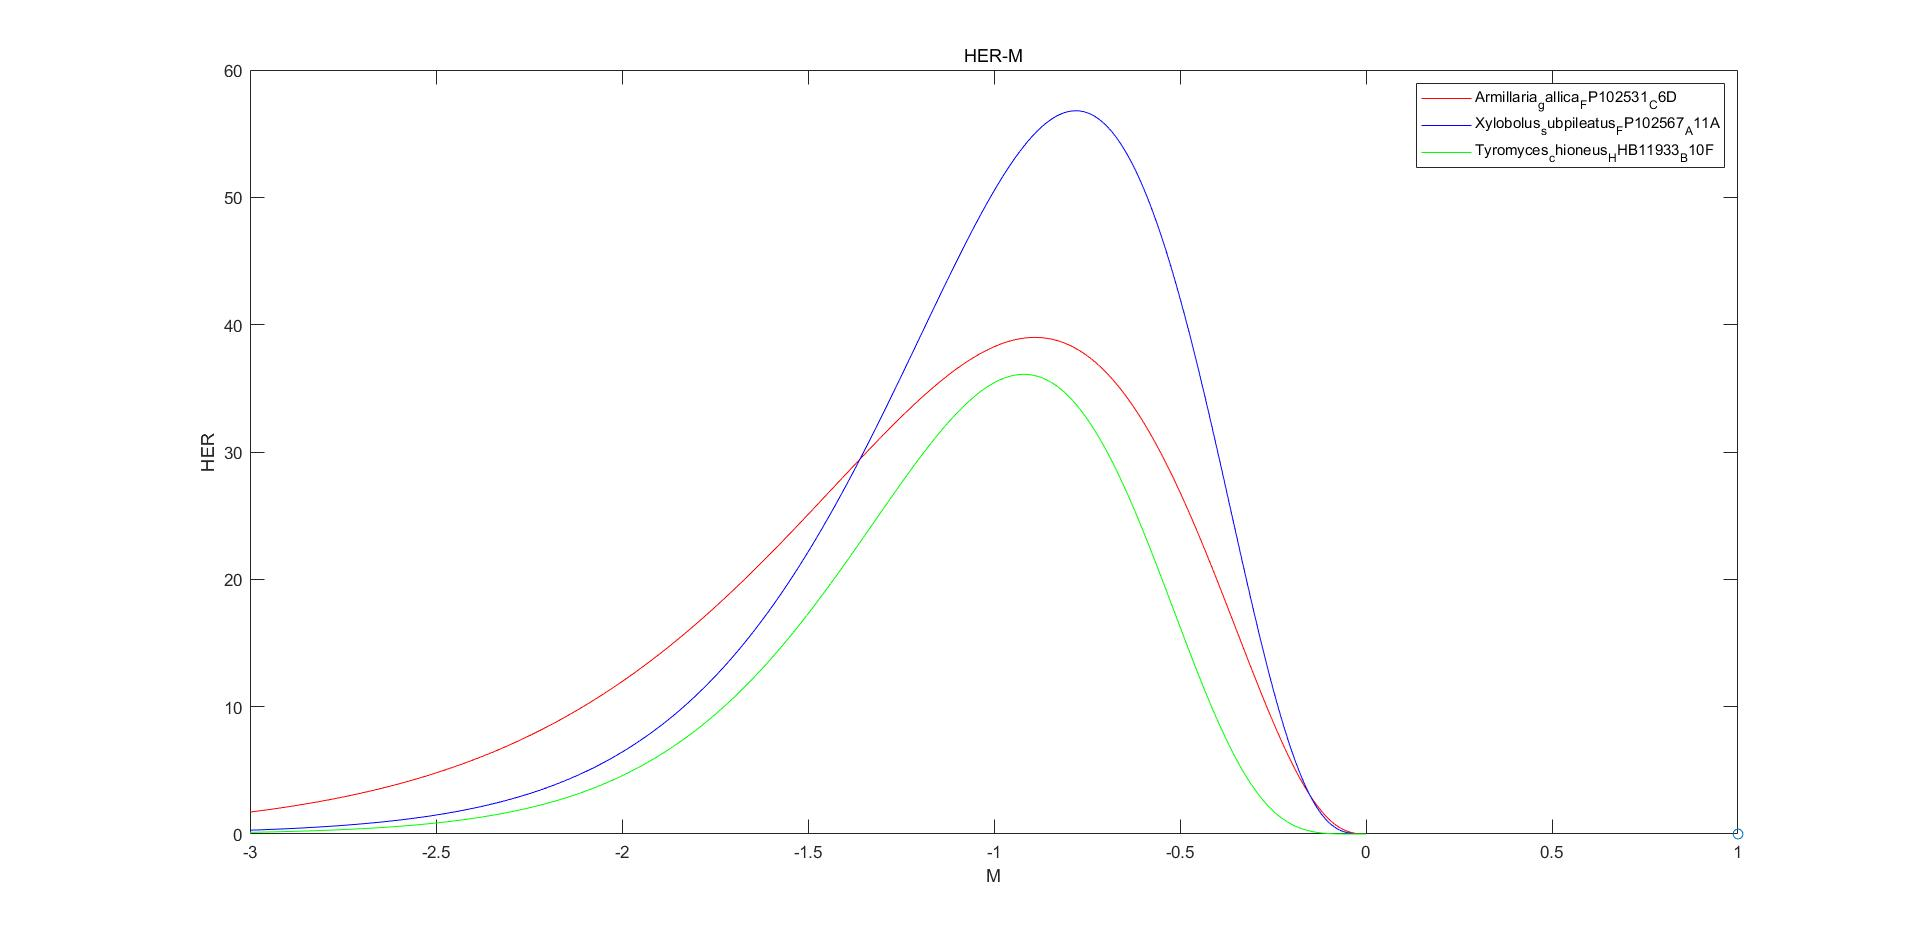
\includegraphics[width=0.8\textwidth]{./picture/HER-M.jpg}}
	\caption{HER-M}
\end{figure}

\newpage
\subsubsection{$MT$-$M_{opt}$ Scatter plot}
Since the moisture tolerance is determined by the population’s competitive ranking and moisture niche width, and through related literature, we find that the population’s optimal moisture is related to its moisture niche width. Therefore, we can think that the population’s optimal moisture and moisture tolerance also exist. There is a certain relationship. The relationship between the 34 populations can be seen in the figure below, which indirectly shows the relationship between humidity and moisture tolerance. Since the moisture tolerance is not greatly affected by temperature, we will not consider it here.
\begin{figure}[h]
	\centering{
		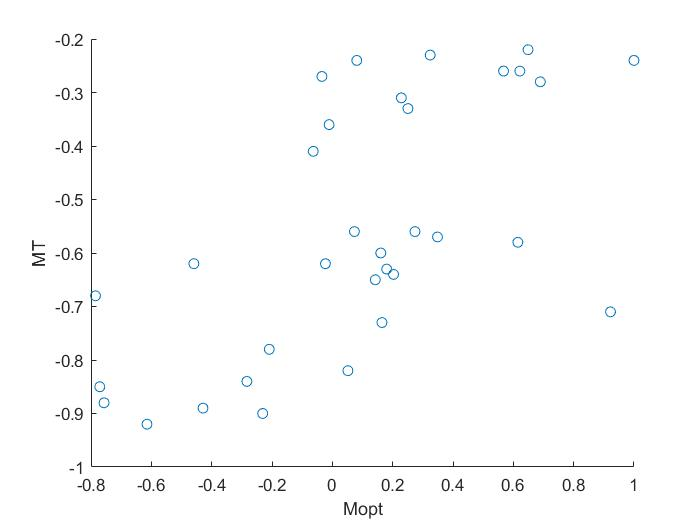
\includegraphics[width=0.6\textwidth]{./picture/MT-Mopt.jpg}}
	\caption{MT-$M_{opt}$}
\end{figure}
\newpage

\subsection{Environmental adaptability under weather changes}
\begin{figure}[h]
	\centering{
		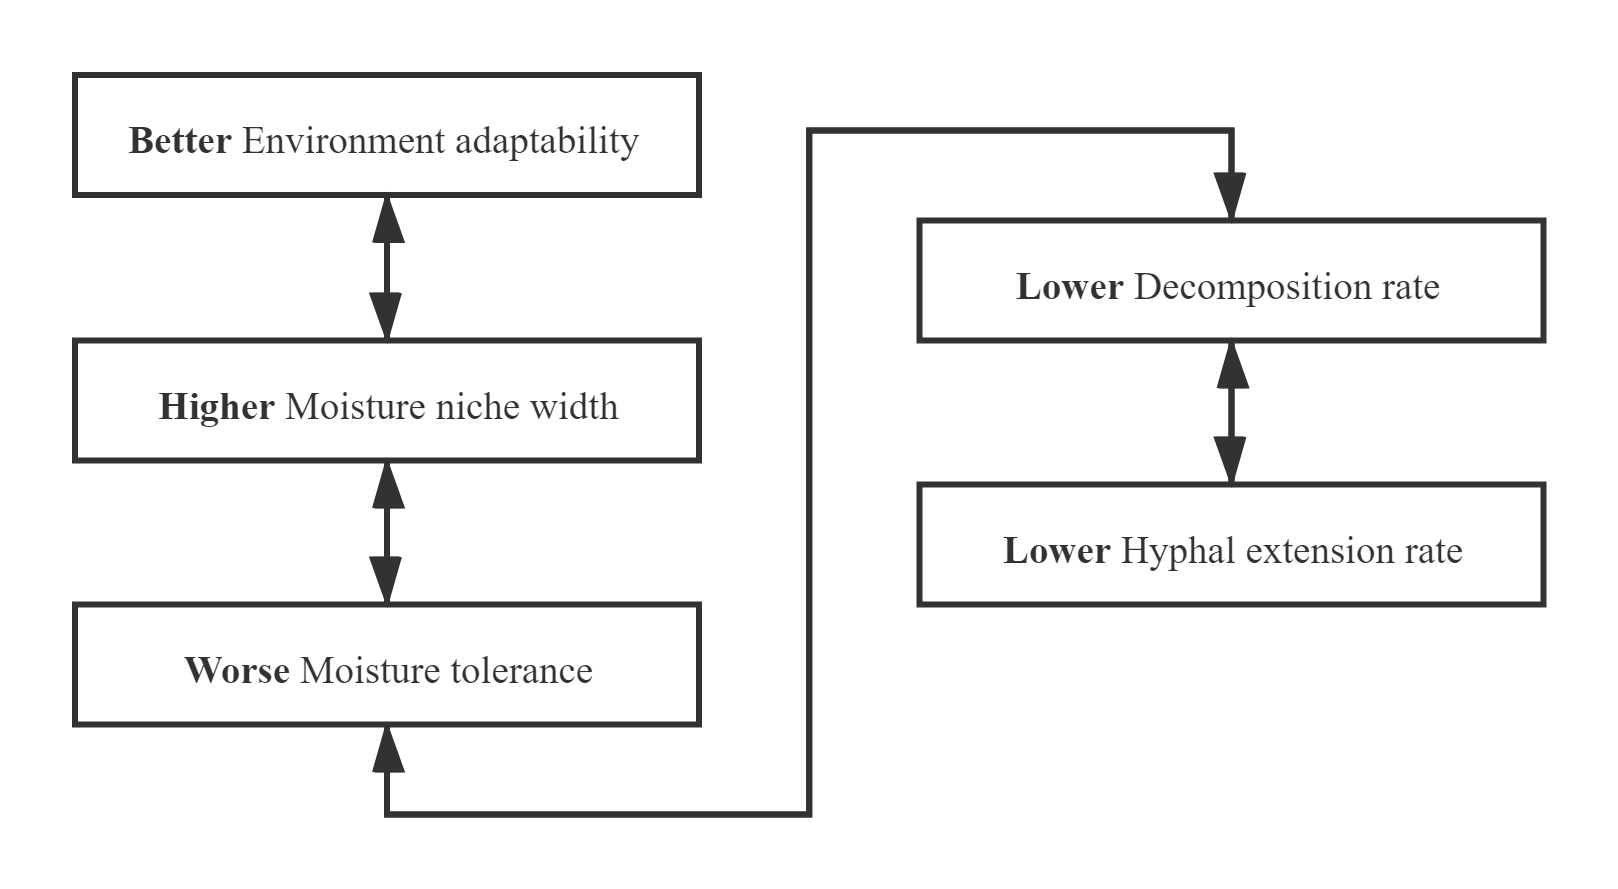
\includegraphics[width=0.8\textwidth]{./picture/impact.png}}
	\caption{impact}
\end{figure}
From the above relationship analysis, we already know that $T$ and $M$ will have a certain impact on the hyphal extension rate and moisture tolerance of the population. In an environment where temperature and humidity change rapidly, different populations have different sensitivity to changing environments. This sensitivity can be reflected by the degree of the impact of environmental changes on the two parameters of the population, which is called the environmental adaptability of the population to different environments. 

Generally speaking, a population with high environmental adaptability has a slower growth rate in a specific environment, while a population with weak environmental adaptability has a very rapid growth and decomposition rate within the adapted environment. This relationship can be inferred from each other, and it is also true from the opposite perspective. The inference relationship of specific effects can be seen in the figure below.

\subsection{Prediction in different environments}
From the previous statement, we know that the hypohal extension rate and moisture tolerance of a single population will be different under different $T$ and $M$, which also means that $T$ and $M$ will affect the population's competitive ranking in this environment. 

Generally speaking, a population with a higher competitive ranking in a certain environment has more development advantages than other populations and can survive the competition of the environment. The advantage of a population with high environmental adaptability is that it can maintain a certain competitive ranking in many environments, can survive in multiple environments, and will not be eliminated. 

But the disadvantages are that such populations tend to grow at a low rate and cannot grow rapidly in a certain environment. For a population with low environmental adaptability, its advantage is that it will become an absolute dominant species in its adapted environment and grow rapidly, but its disadvantage is that it has a low competitive ranking in an environment where it is difficult to adapt, and may compete Was eliminated. 

Next, we introduce a population of six fungi in five different specific environments, and establish a model through the definition and analysis of the competitive ranking value to better illustrate this problem.

\begin{table}[h]
	\centering
	\caption{Five regions with different climates}
	\begin{tabular}{p{.1\textwidth}p{.15\textwidth}p{.15\textwidth}p{.15\textwidth}p{.12\textwidth}p{.13\textwidth}}
		\hline
		Regions&AP($mm$)&DPT($^{\circ}$C)&AT($^{\circ}$C)&RM&AM($kg/m^{3}$)\\
		\hline
		A & 189 &-6.57 & 1.51 & 54.87\% & 3.73\\
		B & 448 &9.39  & 16.37& 63.34\% & 8.33\\
		C & 650 &2.88  & 9.76 & 62.21\% & 5.63\\
		D & 1378 &13.26 & 17.88& 74.42\% & 12.95\\
		E & 1839 &20.29 & 23.39& 82.79\% & 19.56\\
		\hline
	\end{tabular}
\end{table}
%DP:TDew point temperature
%AP:Average precipitation
%AT:Average temperature
%RM:Relative moisture
%AM:Absolute moisture
In the table above,A is Temperate continental climate,B is Monsoon Climate of Medium Latitudes,C is Monsoon Climate of Medium Latitudes,D is Subtropical Monsoon Climate,E is Tropical Monsoon Climate.

We assume that the absolute niche ranking is $R$,and $R$ can be defined by
\begin{equation}
	R=R(r_{1})+R(r_{2})
\end{equation}
where $r_{1}$ is the relative temperature difference value and $r_{2}$ is the relative moisture difference value.

Through the previous discussion,we can define that
\begin{equation}
	r_{1}=\lvert{\frac{T_{opt}-T}{T_{max}-T_{opt}}}\lvert
\end{equation}
and that
\begin{equation}
	r_{2}=\lvert{\frac{M_{opt}-M}{M_{max}-M_{opt}}}\lvert
\end{equation}

Substitute the corresponding values for different fungi,we got different values of $r_{1}$ and $r_{2}$.

Assign the maximum value of $r$ to $0$ of $R(r)$,the minimum value of $r$ to $1$ of $R(r)$.By linear function,we get the one-to-one correspondence between $r$ and $R(r)$.We can clearly see that $r$ and $R(r)$ have a negative correlation and the range of $R(r)$ is$[0,2]$.

According to our definition, we can know that when r is smaller, the relative difference is smaller, R is larger, and the ranking is higher at this time.

\begin{table}[h]
	\centering
	\caption{The value of $R$ in different environments}
	\begin{tabular}{p{.55\textwidth}p{.05\textwidth}p{.05\textwidth}p{.05\textwidth}p{.05\textwidth}p{.05\textwidth}}
		\hline
		Fungi & A & B & C & D & E\\
		\hline
		Schizophyllum\_commune\_PR1117 & 0.48 & 0.66 & 0.97 & 0.43 & 0.53\\
		Fomes\_fomentarius\_TJV93\_7\_A3E & 0.82 & 0.89 & 0.99 & 1.68 & 1.60\\
		Lentinus\_crinitus\_PR2058\_C1B & 0.36 & 0.44 & 0.38 & 0.99 & 1.56\\
		Phellinus\_robiniae\_AZ15\_A10H Banik/Mark & 0.66 & 0.70 & 0.79 & 1.44 & 1.48\\
		Phlebia\_acerina\_DR60\_A8A & 0.90 & 0.65 & 0.87 & 0.77 & 0.71\\
		Phlebiopsis\_flavidoalba\_FP102185\_B12D & 0.97 & 0.88 & 0.92 & 1.30 & 1.62\\
		\hline
	\end{tabular}
\end{table}

The competitive ranking is obtained according to the competitiveness definition value R above. The ranking from 1 to 6 represents the ranking of competitive ability from the largest to the smallest. The results are shown in the following table.
\begin{table}[h]
	\centering
	\caption{The adaptation ranking in different environments}
	\begin{tabular}{p{.55\textwidth}p{.05\textwidth}p{.05\textwidth}p{.05\textwidth}p{.05\textwidth}p{.05\textwidth}}
		\hline
		Fungi & A & B & C & D & E\\
		\hline
		Schizophyllum\_commune\_PR1117 & 5 & 4 & 2 & 6 & 6\\
		Fomes\_fomentarius\_TJV93\_7\_A3E & 3 & 1 & 1 & 1 & 2\\
		Lentinus\_crinitus\_PR2058\_C1B & 6 & 6 & 6 & 4 & 3\\
		Phellinus\_robiniae\_AZ15\_A10H Banik/Mark & 4 & 3 & 5 & 2 & 4\\
		Phlebia\_acerina\_DR60\_A8A & 2 & 5 & 4 & 5 & 5\\
		Phlebiopsis\_flavidoalba\_FP102185\_B12D & 1 & 2 & 3 & 3 & 1\\
		\hline
	\end{tabular}
\end{table}

Competitive ranking is essentially a function of environmental adaptability $ES$ and the difference between environmental conditions and optimal conditions

\subsection{Impact of biodiversity}
In order to illustrate the role of diversity of fungal communities in an entire ecosystem, we will compare six species with a single species as an example, hoping to illustrate the impact of diversity of species.
\subsubsection{The role of diversity in breakdown of ground litter}
In the breakdown of ground litter, we know that its decomposition rate is positively correlated with the growth rate of the fungal population. Through the growth model of the above population and the six-population competition model, we know its decomposition rate when a population exists,it is $0.2022N_{0r}$, and under the same conditions ($N_{0}$ and $r$ are the same), in the six-population competition model constructed above, their total growth rate is about 1.5 times that of a single species, which shows that the decomposition rate of the six-populations will be greater than that of a single population. At the same time, considering the effective decomposition time ($HER>=0.5HER_{max}$), the overall duration of the six populations is also significantly longer than that of the single population. This also shows that the decomposition effect of the six populations on the ground litter is significantly better than the single population, and the efficiency is higher. This also shows that the diversity of fungal populations is conducive to the decomposition of ground litter.
\subsubsection{Stability of diversity in environmental changes}
Through the above prediction models of population changes in different environments, we know that the competitive ranking of a population in different environments will change, that is, the adaptability will be different. Therefore, if there is only one population in an environment, when the environment changes rapidly, its adaptability may decrease, and the $r$ in its growth model may change, its growth rate may decrease, and the population may die out. A population is unstable. On the contrary, if there are multiple populations, just like the six-population model applied above, different dominant species will appear in each environment, and there are populations that can grow stably in the environment, so even if the environment changes, the entire six populations can still maintain a certain level. The growth rate is stable,therefore, the diversity of the fungus population ensures that it has sufficient environmental adaptability as a whole and ensures that it can remain stable in a rapidly changing environment.

\section{Sensitivity analysis}
Our article mainly established a multi-fungal decomposition model in the natural environment. One of the important models is the multi-species competition model based on the logistic model. What we are not sure about in this model is the initial quantity of the various groups. At the beginning, for the sake of simplicity, we assumed that the number of various groups was 10\% of the maximum. But in reality, the number of various groups will only be close to not exactly the same proportion. Now, in order to better explain the rationality of this assumption, we use the change of the initial quantity to do a sensitivity analysis of the relevant model. Make slight adjustments to the initial quantities of different populations, and on the basis of the model, the following curve comparison chart can be obtained:
\begin{figure}[h]
	\centering{
		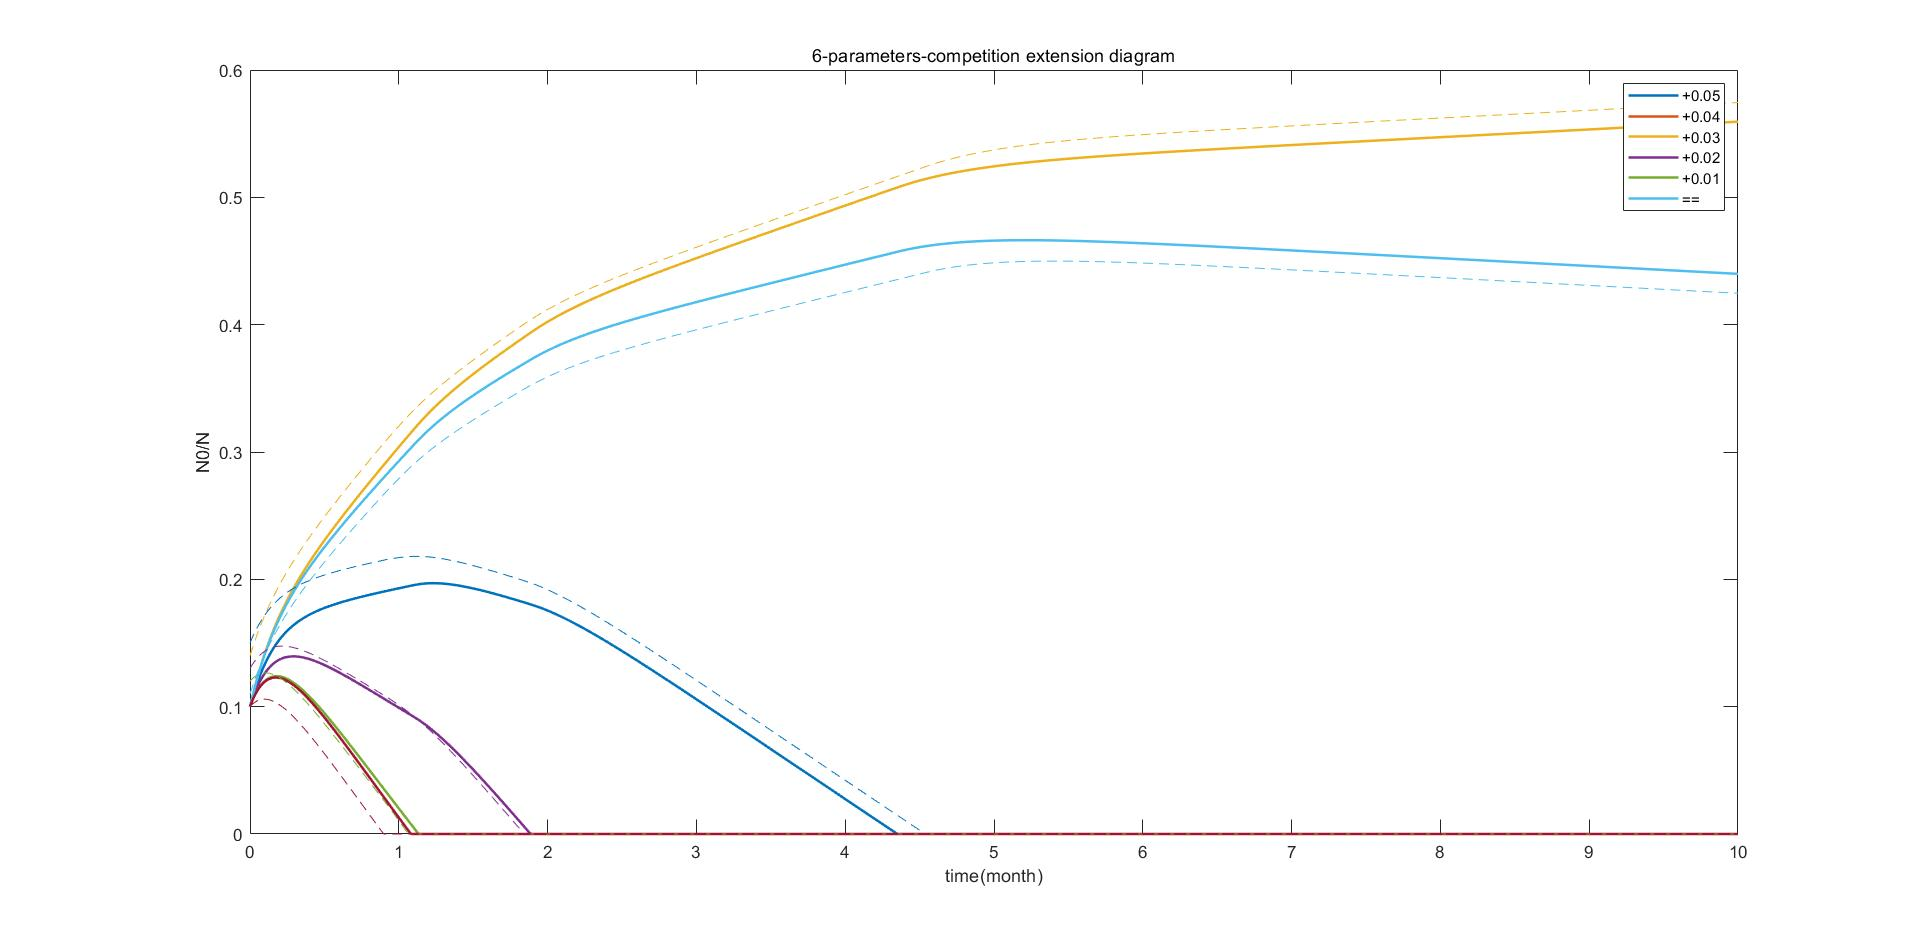
\includegraphics[width=0.8\textwidth]{./picture/sensitivity.jpg}}
	\caption{Sensitivity}
\end{figure}

From the comparison chart, we find that under the condition of small changes in the initial quantity, the trend of the curve afterwards does not change much, and all conclusions and analyses are still valid. This shows that the model has little dependence on the initial value conditions and is a relatively stable model under reasonable assumptions.

\section{Strengths and Weaknesses}

\subsection{Strengths}
\begin{itemize}
	\item
	Our model has real and credible data sources, most of which are collected in various professional papers and professional databases.
	\item 
	Our model is formulated on a certain theoretical basis. After consulting a lot of professional papers, we carefully selected the parameters of the model. In this way ,we can make our model as close to reality as possible.
	\item 
	We made reasonable assumptions to simplify the problem. For the difficult-to-handle hyphal extension rate, we use the logistic model to explain; and for the complex relationship,we adopt a linear fitting method based on the least square method to determine.  
	\item 
	We considered several climatic conditions in reality and applied our model under these climatic conditions. 
	\item 
	We do a sensitivity analysis of the model , which illustrates the relative stability of the model and the rationality of some of our assumptions.
\end{itemize}

\subsection{Weaknesses}
\begin{itemize}
	\item 
	We are not complete when considering the factors that affect the decomposition rate. We attribute the main environmental factors to only temperature and humidity.
	\item 
	In the process of data relationship processing, we express the binary relationship of the data through function fitting, which often has certain errors. The results obtained by the model may be different from the true value. 
	\item 
	Our model is considered within limited conditions, which may not be suitable for some specific situations.
\end{itemize}

\begin{thebibliography}{10}  
	\bibitem{ref1}Lustenhouwer N, Maynard DS, Bradford MA, Lindner DL, Oberle B, Zanne
	AE, Crowther TW. 2020. A trait-based understanding of wood decomposition by fungi. Proc Natl Acad Sci USA 117:11551-11558.
	\bibitem{ref2}D. S. Maynard et al., Consistent trade-offs in fungal trait expression across broad spatial scales. Nat. Microbiol. 4, 846–853 (2019).
	\bibitem{ref3}Dang, Christian K and Schindler, Markus and Chauvet, Eric and Gessner, Mark O Temperature oscillation coupled with fungal community shifts can modulate warming effects on litter decomposition. (2009) Ecology, vol. 90 (1). pp. 122-31.
	ISSN 0012-9658.
	\bibitem{ref4}Glassman, S.I., Weihe, C., Li, J., Albright, M.B., Looby, C.I., Martiny, A.C. et al. (2018),Decomposition responses to climate depend on microbial community composition. PNAS 115:11994-11999. 
	\bibitem{ref5}Větrovský, T., P. Kohout, M. Kopecký, A. Machac, M. Man, et al. (2019). A meta-analysis of global fungal distribution reveals climate-driven patterns. Nature Communications 10:1-9.
	\bibitem{ref5}Giauque, H., and C. V. Hawkes.(2013). Climate affects symbiotic fungal endophyte diversity and performance. American Journal of Botany 100:1435-1444.
\end{thebibliography}
\newpage
\begin{center}
	\LARGE
	\textbf{The role of Fungi in Ecological systems}
\end{center}

As we all know, fungi are important part of the ecosystem.Fungi affect the cycle of organic matter by participating in the enzymatic degradation process of litter, and affect the inorganic cycle of nitrogen, phosphorus, potassium, calcium, magnesium and other elements by promoting biological nitrogen fixation, accelerating soil phosphorus weathering, improving the availability of soil solution ions and direct absorption.

\begin{figure}[h]
	\centering 
	\subfigure[Fungi under the camera]{
		\label{Fig.sub.1}
		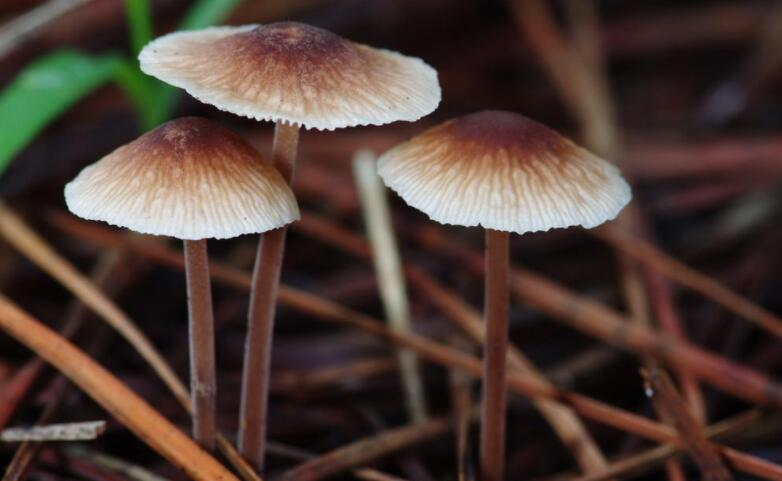
\includegraphics[width=0.45\textwidth]{fungus1.jpg}}
	\subfigure[Fungi under the microscope]{
		\label{Fig.sub.2}
		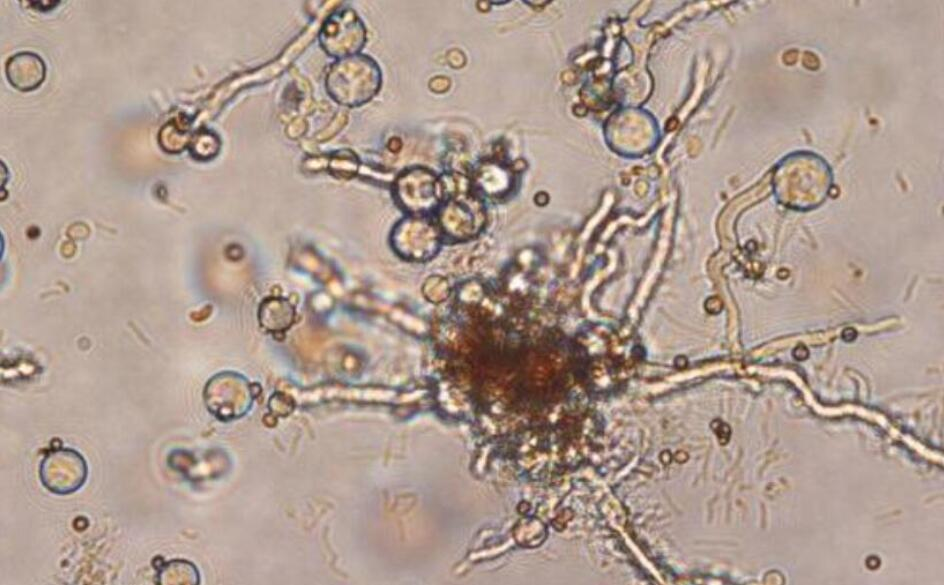
\includegraphics[width=0.45\textwidth]{fungus2.jpg}}
\end{figure}

Especially, the effects of fungi on the ecosystem are realized through breakdown of ground litter and woody fibers.Our work have found that the decomposition rate(DR) is closely related to two traits of a fungus: the hyphal extension rate of the fungus(HER) and the fungus’ tolerance to moisture(MT).Based on a large amount of data, we fit the relationship curve between decomposition rate and growth rate (as shown in the left figure below), and they are roughly logarithmic. In the meantime,we fit the relationship curve between decomposition rate and moisture tolerance(as shown in the right figure below), and they are roughly logarithmic.

\begin{figure}[h]
	\centering 
	\subfigure[DR-HER Curve]{
		\label{Fig.sub.3}
		\includegraphics[width=0.45\textwidth]{DR-HER.jpg}}
	\subfigure[DR-MT Curve]{
		\label{Fig.sub.4}
		\includegraphics[width=0.45\textwidth]{DR-MT.jpg}}
\end{figure}

The above results are obtained in the same environment. Since the decomposition rate is different in different environments, our work also explores the influence of the environment on the decomposition rate. In this regard, we believe that the temperature and moisture in environmental factors indirectly affect the decomposition rate by affecting the hyphal extension rate and moisture tolerance.Each fungi population has its own unique optimal temperature and optimal moisture, and will reflect different competitive characteristics and environmental adaptability in different environments.

Furthermore, our work illustrates the role of fungal population diversity in ecosystems.Firstly,we established a single population and multiple population growth models. The specific changes based on the logistic model can be seen in the figure below.
\begin{figure}[h]
	\centering 
	\subfigure[Single-logistic Model]{
		\label{Fig.sub.5}
		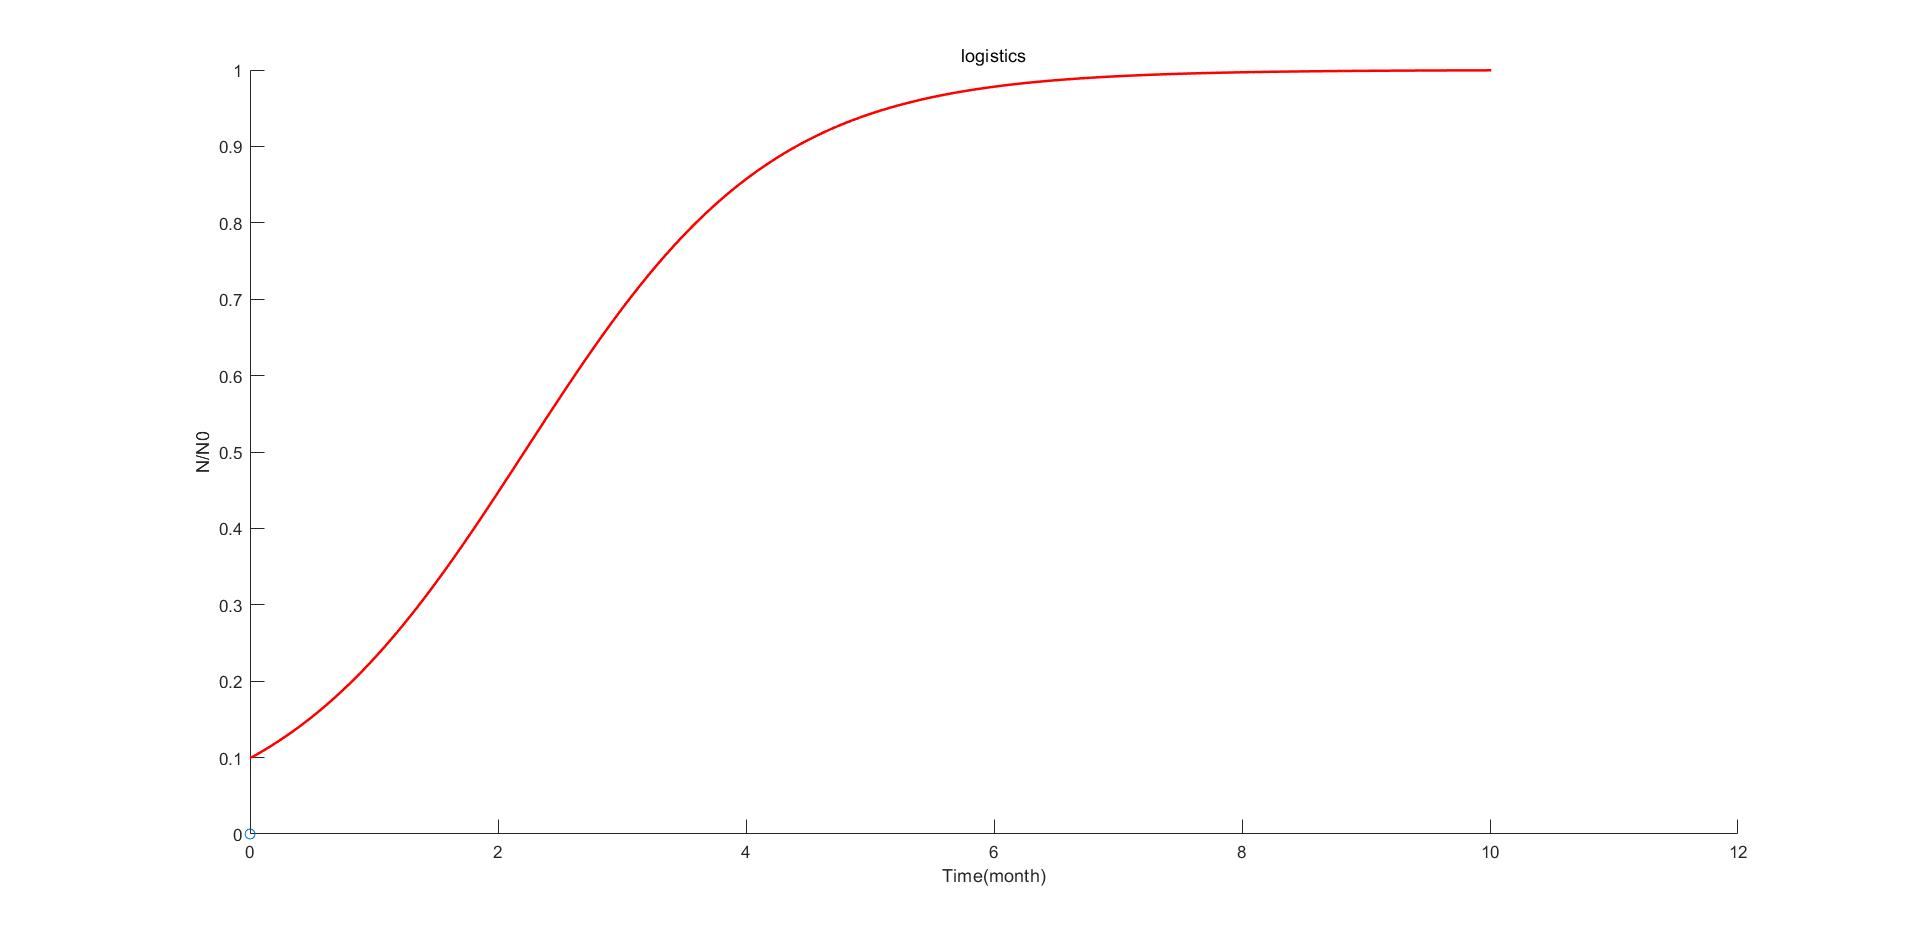
\includegraphics[width=0.55\textwidth]{single-logistic.jpg}}
	\subfigure[Competition Model]{
		\label{Fig.sub.6}
		\includegraphics[width=0.35\textwidth]{competition.jpg}}
\end{figure}

From the above model, we conclude that the total growth rate of multiple populations is 1.5 times that of a single population, and its decomposition rate is correspondingly much faster than that of a single population. Multiple fungal populations are more helpful for decomposition of ground litter.Additionally, through the analysis of environmental adaptability, we found that the environmental adaptability of multiple fungal populations is significantly higher. The diversity of population types can make it maintain a certain decomposition rate and maintain stability in various rapidly changing environments.
\begin{figure}[h]
	\centering 
	\subfigure[Decomposition of fungi(1)]{
		\label{Fig.sub.1}
		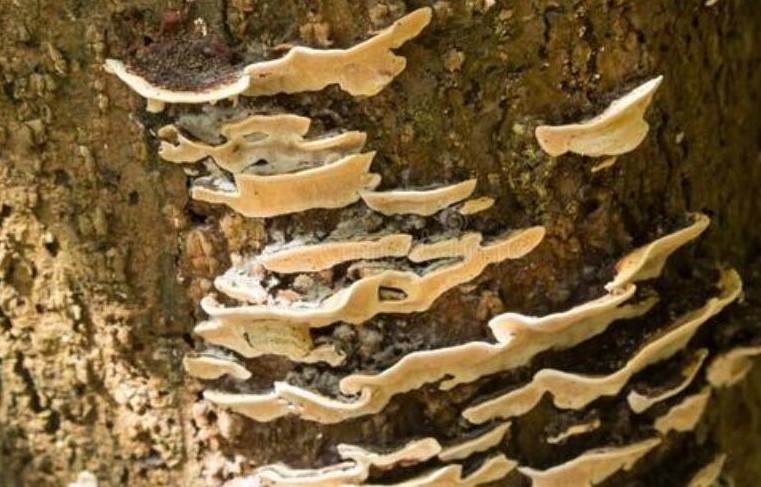
\includegraphics[width=0.42\textwidth]{decomposition1.jpg}}
	\subfigure[Decomposition of fungi(2)]{
		\label{Fig.sub.2}
		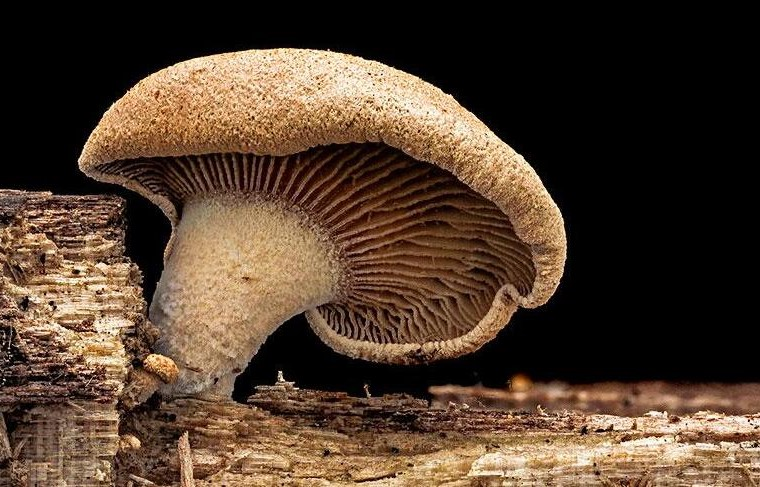
\includegraphics[width=0.42\textwidth]{decomposition2.jpg}}
\end{figure}

In summary, we believe that fungi mainly act as decomposers in the ecosystem. Its decomposition rate is affected by a variety of population characteristics and environmental factors. The diversity of the fungus population can help it better adapt to the environment and perform its decomposition more efficiently.

\newpage
\begin{appendices}
\section{First appendix}
\begin{table}[h]
	\centering
	\caption{Moisture tolerance - Decomposition rate - Optimal moisture}
	\begin{tabular}{p{.55\textwidth}p{.1\textwidth}p{.1\textwidth}p{.1\textwidth}}
		\hline
		$gen.name$ & $MT$ & $DR$ & $M_{opt}$ \\ 
		\hline
		Armillaria\_gallica\_FP102531\_C6D & -0.429  & 4.07  & 2.57 \\
		Armillaria\_gallica\_EL8\_A6F & -0.209  & 3.20  & 1.77 \\ 
		Armillaria\_gallica\_FP102534\_A5A & -0.614  & 2.94  & 3.26 \\
		Armillaria\_gallica\_FP102535\_A5D & -0.771  & 3.78  & 3.79 \\ 
		Armillaria\_gallica\_FP102542\_A5B & -0.231  & 2.35  & 2.19 \\ 
		Armillaria\_gallica\_HHB12551\_C6C & -0.785  & 2.03  & 3.66 \\ 
		Armillaria\_gallica\_OC1\_A6E & -0.283  & 2.29  & 2.01 \\ 
		Armillaria\_gallica\_SH1\_A4A & -0.063  & 2.18  & 1.80 \\ 
		Armillaria\_sinapina\_PR9 & -0.011  & 1.72  & 1.53 \\ 
		Armillaria\_tabescens\_FP102622\_A3C & -0.459  & 3.56  & 3.03 \\ 
		Armillaria\_tabescens\_TJV93\_261\_A1E & -0.034  & 2.83  & 1.16 \\ 
		Fomes\_fomentarius\_TJV93\_7\_A3E & 0.081  & 10.41  & 1.05 \\ 
		Hyphodontia\_crustosa\_HHB13392\_B7B & 0.324  & 4.29  & 1.05 \\ 
		Hyphoderma\_setigerum\_HHB12156\_B3H & 0.568  & 5.64  & 1.05 \\ 
		Hyphoderma\_setigerum\_FP150263\_B2C & 0.274  & 2.67  & 1.18 \\ 
		Laetiporus\_conifericola\_HHB15411\_C8B & 0.073  & 2.29  & 0.96 \\ 
		Lentinus\_crinitus\_PR2058\_C1B & 0.229  & 3.47  & 1.37 \\
		Mycoacia\_meridionalis\_FP150352\_C4E & 0.324  & 2.16  & 1.05 \\
		Merulius\_tremullosus\_FP102301\_C3E & 0.622  & 22.78  & 1.05 \\ 
		Merulius\_tremellosus\_FP150849\_C3F & 0.689  & 13.52  & 1.10 \\ 
		Phlebiopsis\_flavidoalba\_FP102185\_B12D & 0.251  & 11.18  & 1.39 \\ 
		Phlebiopsis\_flavidoalba\_FP150451\_A8G & 0.615  & 6.40  & 2.23 \\ 
		Phellinus\_gilvus\_HHB11977\_C4H & 0.161  & 5.15  & 1.11 \\ 
		Phellinus\_hartigii\_DMR94\_44\_A10E & 0.142  & 2.30  & 1.34 \\ 
		Porodisculus\_pendulus\_HHB13576\_B12C & 0.203  & 2.61  & 0.94 \\ 
		Phellinus\_robiniae\_FP135708\_A10G & 0.180  & 3.68  & 1.21 \\ 
		Phellinus\_robiniae\_AZ15\_A10H Banik/Mark & -0.023  & 2.22  & 1.17 \\ 
		Phlebia\_acerina\_MR4280\_B9G & 1.000  & 11.88  & 1.05 \\ 
		Phlebia\_acerina\_DR60\_A8A & 0.922  & 5.97  & 0.91 \\ 
		Pycnoporus\_sanguineus\_PR\_SC\_95\_A11C & 0.349  & 4.44  & 1.51 \\ 
		Schizophyllum\_commune\_TJV93\_5\_A10A & 0.165  & 3.92  & 1.94 \\ 
		Schizophyllum\_commune\_PR1117 & 0.052  & 2.55  & 1.92 \\ 
		Tyromyces\_chioneus\_HHB11933\_B10F & 0.649  & 5.35  & 1.05 \\ 
		Xylobolus\_subpileatus\_FP102567\_A11A & -0.757  & 2.17  & 4.37 \\ 
		\hline
	\end{tabular}
\end{table}
\newpage
\section{Second appendix}
Data source websites:
\begin{itemize}
	\item 
	AVIATION WEATHER CENTER, \href{}{https://aviationweather.gov/}
	\item 
	fungal\_biogeography, GitHub, \href{}{https://github.com/dsmaynard/fungal\_biogeography} 
	\item
	PNAS, https://www.pnas.org/content/suppl/2020/05/13/1909166117.DCSupplemental
\end{itemize}

Data source tools:
\begin{itemize}
	\item 
	WheatA, Big Data of Agricultural Meteorology
\end{itemize}

\end{appendices}
\end{document}
